% 
%Descripción del sistema
%	Arquitectura del sistema
%	Recolección y almacenamiento de datos
%	Detección de eventos sísmicos
%		Monitoreo de la Velocidad Relativa
%		Metodología para ajuste de parámetros óptimos
%	Geocodificación de los datos
%	Visualizaciones
%		Temporales
%		Geográficas
%	Aplicación Web
%

\chapter{Descripción del sistema}
\label{cap:sistema}

En esta tesis se propone un sistema capaz de detectar sismos en el mundo a partir de los datos publicados en Twitter y una aplicación Web para visualizar en tiempo real la información extraída de los datos. También se busca realizar análisis con los datos para comparar el modelo de detección con el estado del arte. 

Para la implementación del sistema de detección de sismos se utiliza una adaptación del modelo propuesto por Guzmán y Poblete~\cite{guzman2013line}. El modelo propuesto por Guzmán y Poblete detecta automáticamente el aumento explosivo en el uso de palabras clave específicas en los mensajes que componen el \textit{stream} de Twitter. La detección se basa en la comparación de la velocidad en la que se publican mensajes que mencionan una palabra clave con respecto a la velocidad ``normal'' de publicación de mensajes que mencionan esa palabra en específico. El modelo tiene buenos resultados sin la necesidad de una etapa de entrenamiento previa que implique tener datos etiquetados y es tolerante al ruido, convirtiéndolo en un buen candidato para ser utilizado en un sistema de detección global o que utilice como \textit{input} mensajes escritos en varios idiomas. El modelo y las modificaciones que se aplicaron para su uso para detección de sismos se explican en detalle en la sección \ref{sec:deteccion}.

En las siguientes secciones se explica la arquitectura general del sistema implementado y con más detalle el funcionamiento de las diferentes partes que lo componen, las que se encargan de recolectar los datos, detectar anomalías, extraer información relevante y visualizar la información. 


\section{Arquitectura}
\label{sec:arquitectura}

\begin{figure}[h]
	\centering
	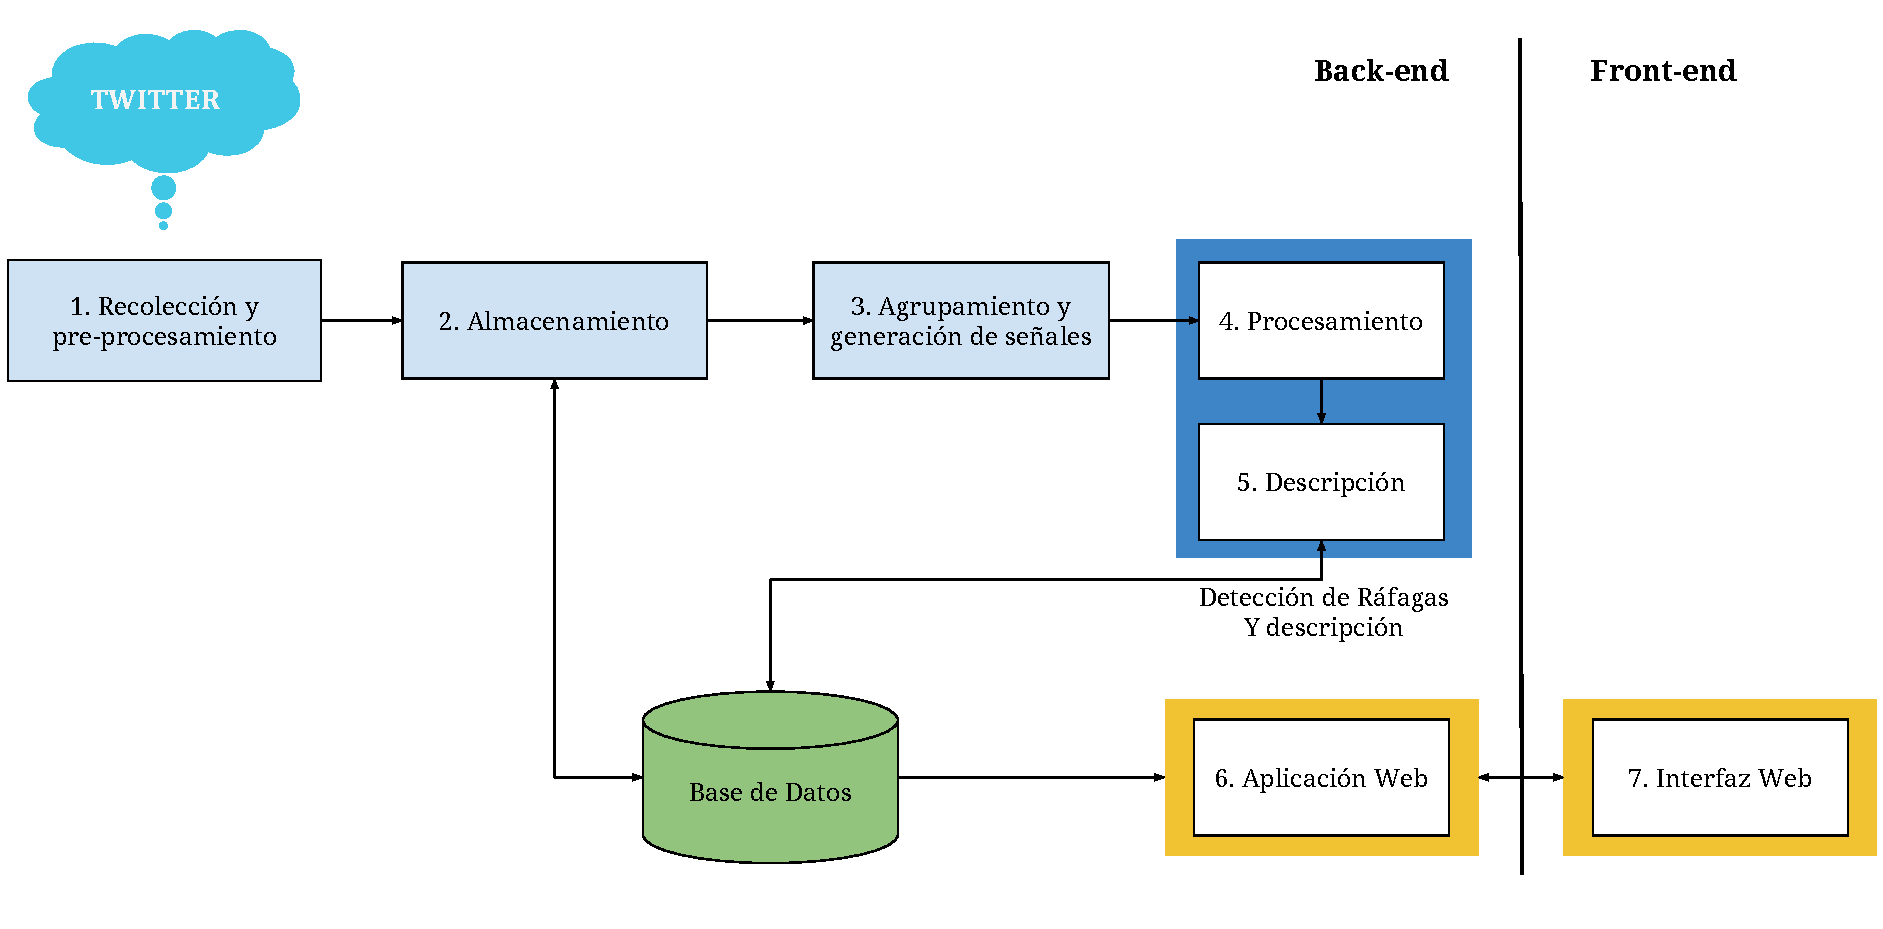
\includegraphics[width=\linewidth]{imagenes/Arquitectura.pdf}
	\caption{Arquitectura del sistema completo}
	\label{img:arquitectura}
\end{figure}

La figura \ref{img:arquitectura} es un esquema de los módulos que conforman el sistema y la forma en que cada uno interactúa con los demás. 
%
Cabe destacar que la experimentación fue una parte importante de este trabajo de tesis. Es por esto que algunos de los procesos generan información que fue evaluada durante la etapa de análisis y que, en base a los resultados obtenidos, no se incluyó en las visualizaciones. 
%
Sin embargo toda la información generada quedó almacenada de forma ordenada para investigaciones futuras. 


A continuación se explican en detalle la función de cada uno de los módulos y las herramientas utilizadas para su implementación: 


\noindent\textbf{1) Recolección de datos y pre-procesamiento}

El módulo 1 se encarga de recibir el flujo de \textit{tweets} a medida que estos son publicados en la red social. 
%
Para obtener los datos se utiliza la API para acceder al \textit{stream} público de Twitter\footnote{\url{https://dev.twitter.com/streaming/public}} y una librería en Java\footnote{\url{http://twitter4j.org/}} que integra el servicio con la aplicación.
%
Los datos se reciben en formato JSON\footnote{\url{https://dev.twitter.com/docs/tweet-entities}}.

Los \textit{tweets} recolectados reciben un primer procesamiento encargado de agregar metadatos a partir del texto y de otras características del \textit{tweet}. El pre-procesamiento de los datos incluye:
\begin{itemize}
\item La ejecución del algoritmo SentiStreigth\footnote{\url{http://sentistrength.wlv.ac.uk}} para calcular el sentimiento del mensaje.
\item La búsqueda de menciones de nombres de países en diferentes idiomas en el mensaje y en los campos que incluyen información de localidad del usuario.
\item Etiquetado de \textit{tweets} de carácter posiblemente malicioso o casos particulares que perturban el correcto funcionamiento de la detección. Se marcan los \textit{tweets} publicados por el mismo usuario en un lapso menor a 5 minutos y también \textit{tweets} publicados por usuarios incluidos en una lista negra. La lista negra existe para casos particulares en que se detecten usuarios cuyas publicaciones entorpezcan el correcto funcionamiento de la aplicación (como fue el caso de una cuenta mexicana que todos los días publicaba la lista completa de sismos del día anterior). Esta lista puede ser actualizada sin necesidad de interrumpir los procesos. 
\end{itemize}

Los metadatos añadidos fueron parte importante del análisis experimental desarrollado. Se detalla un poco más sobre el proceso de extracción de sentimiento en la sección \ref{sec:sentimiento} y sobre el proceso de geolocalización en la sección \ref{sec:geocodificacion}. Además en el capítulo \ref{cap:analisis} se explica cómo se utilizaron estos datos en el análisis experimental y los resultados obtenidos.

Finalmente, luego de procesar cada \textit{tweet}, este es encolado en memoria caché para ser utilizado por el módulo 2.

\noindent\textbf{2) Almacenamiento de datos}

\begin{figure}[ht]
	\centering
	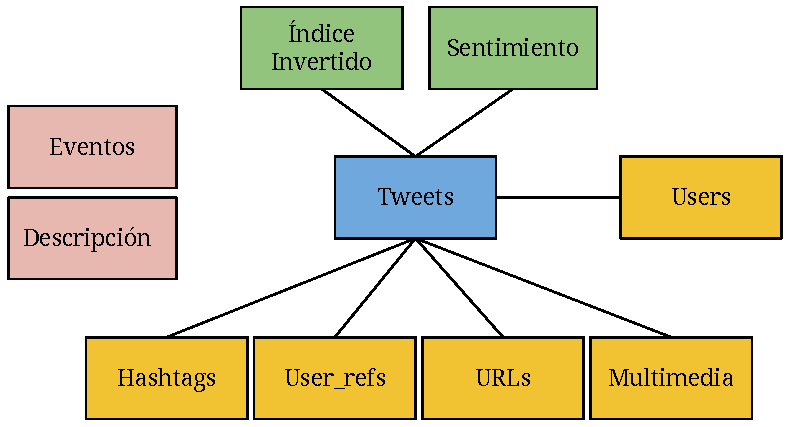
\includegraphics[width=0.8\linewidth]{imagenes/tweetmodel.pdf}
	\caption{Modelo de las tablas generadas diariamente que conforman la base de datos.}
	\label{img:database}
\end{figure}

El módulo 2 se encarga del almacenamiento de los \textit{tweets} recolectados y los metadatos asociados. La información se almacena en una base de datos relacional MySQL. 
%
Cada día se crean nuevas tablas para almacenar la información. Esta medida busca evitar tablas de gran tamaño y así optimizar los tiempos de búsqueda en la base de datos. 


La imagen \ref{img:database} muestra las tablas generadas diariamente. 
%
Las tablas de color amarillo almacenan información relacionada al \textit{tweet}. 
%
Los campos de estas tablas guardan información, en su mayoría, proveniente directamente desde Twitter.
%
Algunos de los datos almacenamos en estas tablas son generados en el módulo de pre-procesamiento, como la información de geolocalización y una etiqueta que indican si el \textit{tweet} fue publicado por un mismo usuario en un corto periodo de tiempo.
%
Las tablas de color verde almacenan otra información generada por el sistema.
%
Una de ellas almacena un índice invertido de las palabras que conforman el texto de los \textit{tweet} y la otra almacena el resultado del análisis de sentimiento para cada \textit{tweet}. 
%
Las tablas de color rosado almacenan la información relacionada con las detecciones y son pobladas con la información generada en los módulos 4 y 5 que se describen más adelante. 


Además de las tablas del modelo de la figura~\ref{img:database}, existen otras ``tablas virtuales'' o ``vistas'' destinadas al almacenamiento de datos agregados que son utilizados para la detección de ráfagas y para el almacenamiento de datos precalculados para las visualizaciones.
%
En el anexo \ref{anexo:database} se detalla el esquema de la base de datos y los campos que conforman cada tipo de tabla creada.

\noindent\textbf{3) Agrupamiento de \textit{tweets} y generación de señales}

El módulo 3 se encarga de preparar los datos para ser procesados en busca de ráfagas.
%
Los \textit{tweets} del \textit{stream} son agrupados en conjuntos etiquetados según el \textit{timestamp} de la fecha de creación. 
%
Cada conjunto de \textit{tweets} representa una ventana de tiempo individual. 
%
Las ventanas de tiempo son alineadas secuencialmente.
%
Cada secuencia de ventanas puede ser representada como una señal discreta, la que posteriormente es analizada en el módulo 4. 
%
Como parte de la experimentación se generaron diferentes tipos de señales a partir de algunos atributos de interés específicos. %Por ejemplo, señales conformadas por tweets que mencionaban un mismo país en el mensaje. 
%
Las señales a modo de experimentación fueron:

\begin{enumerate}
\item Señal de \textit{tweets} con palabras clave: Señal conformada por todos los \textit{tweets} que contienen cualquier palabra relacionada con sismos en cualquier idioma~\footnote{Palabras especificadas en una lista de palabras clave.}. 
\item Señales de localización del usuario: Señales construídas mediante la agrupación de tweets publicados por usuarios que indican pertenecer al mismo país en su perfil. Para esto se consideran los \textit{tweets} que contienen palabras relacionadas con sismos.
\item Señales de localización considerando el texto: Señales construídas mediante la agrupación de \textit{tweets} que mencionan el mismo país en el texto del mensaje. Para esto se consideran los \textit{tweets} que contienen palabras relacionadas con sismos.
\item Señales de idioma: Señales construídas mediante la agrupación de \textit{tweets} escritos en el mismo idioma. Para esto se consideran los \textit{tweets} que contienen palabras relacionadas con sismos.
\item Señales de sentimiento: Dos señales, una que agrupa los \textit{tweets} que reportan sismos y que expresan sentimiento positivo y otra con los \textit{tweets} que reportan sismos y que expresan sentimiento negativo. 
\end{enumerate}

Las diferentes señales creadas y los resultados obtenidos a partir de su análisis para detección de sismos se detallan en el capítulo\ref{cap:analisis}.

\noindent\textbf{4) Procesamiento}

El módulo 4 se encarga de procesar las secuencias de ventanas generadas por el módulo anterior y analizarlas en busca de ráfagas.  
%
Para analizar los datos se utiliza una estructura de datos de tabla de hash concurrente en donde se almacenan datos estadísticos asociados a cada ventana de tiempo. Esta estructura permite acceder a los datos en paralelo y mejorar el rendimiento.
%
En la sección \ref{sec:deteccion} se explica en más detalle el algoritmo utilizado para la detección de ráfagas.

\noindent\textbf{5) Descripción}

El módulo 5 se encarga de la descripción de eventos, es decir, se encarga de procesar la ventana de tiempo donde se detectó una ráfaga para determinar las palabras y los \textit{tweets} que propiciaron ese comportamiento.
%
Con esta información se complementa la información temporal y geográfica asociada a esa ventana de tiempo.
%
En conjunto toda esta información describe un evento, ya que responden a las preguntas sobre el cuándo, dónde y qué es lo que pasó específicamente en cada evento detectado.


\noindent\textbf{6) Aplicación Web}

El módulo 6 corresponde al servidor de la aplicación Web implementado en Python utilizando el \textit{framework} Flask\footnote{\url{http://flask.pocoo.org/}}. El servidor accede directamente a la base de datos y consulta los datos a medida que estos van siendo agregados. Para servir los datos en tiempo real se utiliza un caché con auto-refresco de 1 segundo, que evita sobrecargar el servidor cuando acceden muchas personas al mismo tiempo a la aplicación. 

\noindent\textbf{7) Interfaz}

El módulo 7 corresponde a la interfaz de la aplicación Web. Para su implementación se utilizaron las siguientes librerías:
\begin{itemize}
\item JQuery.js\footnote{\url{https://jquery.com/}}: Librería javascript para facilitar la manipulación de documentos y las llamadas Ajax. 
\item Bootstrap\footnote{\url{http://getbootstrap.com/}}: Framework para desarrollar aplicaciones responsivas y que funcionan en varios dispositivos.
\item D3.js\footnote{\url{https://d3js.org/}}: Librería javascript para manipular documentos basados en datos y generar visualizaciones interactivas. %
\item Leaflet.js\footnote{\url{http://leafletjs.com/}}: Librería javascript para visualizaciones interactivas usando mapas. 
\item Leaflet.heat\footnote{\url{https://github.com/Leaflet/Leaflet.heat}}: Un plugin que extiende Leaflet para crear mapas de calor. 
\item Leaflet.markercluster\footnote{\url{https://github.com/Leaflet/Leaflet.markercluster}}: Un plugin que extiende Leaflet para agrupar marcadores cercanos entre si y desplegarlos de forma interactiva. 
\end{itemize}

En la sección \ref{sec:visualizacion} se detallan las visualizaciones utilizadas para presentar los datos y en la sección \ref{sec:aplicacion} se muestran vistas completas de la aplicación y su modo de uso. 

\section{Recolección de Datos}
\label{sec:recoleccion}

Twitter tiene dos servicios para acceder a los datos públicos: 
%
La API de búsqueda, que permite realizar consultas usando palabras clave, idioma, coordenadas geográficas, etc. 
%
Y la API para acceder al \textit{stream} público y que permite obtener el flujo de \textit{tweets} publicados en tiempo real filtrado por palabras clave, idioma, etc.
%
La principal diferencia entre ambas son las limitaciones, ya que la API de búsqueda permite hacer una cantidad limitada de consultas por minuto y la API del \textit{stream} limita la muestra de datos entregada para que no exceda al 1\% del total de mensajes publicados en Twitter en ese momento.
% 
Para este caso, a diferencia de Sakaki et al.\cite{sakaki2013tweet}, Robinson et al. \cite{robinson2013sensitive} y Earle et al. \cite{earle2012twitter}, se decidió ocupar la API para acceder al \textit{stream} público, como también lo hacen Avennuti et. al \cite{avvenuti2014earthquake}.
%
Mediante el uso de la API para acceder al \textit{stream} es posible obtener los \textit{tweets} más rápido y detectar en tiempo más cercano al ``tiempo real''. %Además, los filtros que se utilizaron para obtener los datos disminuyen el número de \textit{tweets} y según nuestra apreciación, la limitante que impone Twitter sobre la muestra de los datos no alcanza a ser suficientemente ajustada como para evitar que se obtengan todos los \textit{tweets} de interés. 

\begin{wrapfigure}{r}{0.5\textwidth}
	\vspace{-20px}
  \centering
    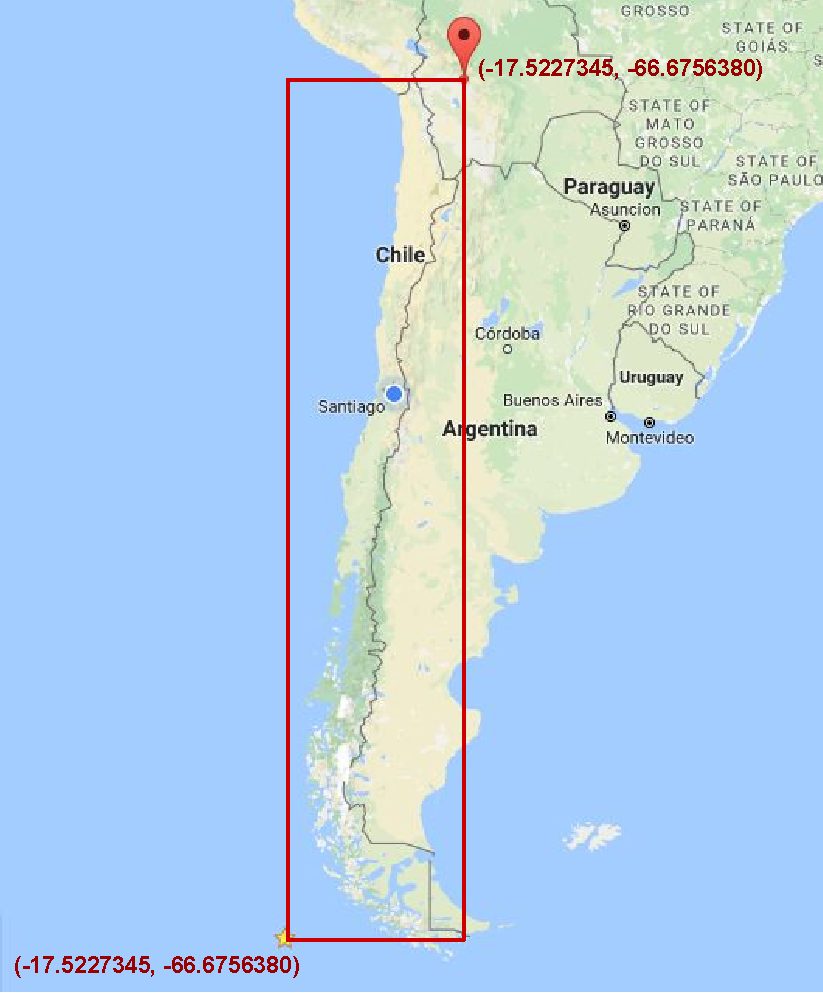
\includegraphics[width=0.48\textwidth]{imagenes/boundingbox.pdf}
  \caption{Cuadro de delimitación geográfica utilizado para recolectar \textit{tweets} de Chile.}
  \label{img:boundingbox}
  \vspace{-10px}
\end{wrapfigure}

Para obtener los datos, se filtró el flujo de mensajes para obtener todos los \textit{tweets} que mencionan alguna de las palabras clave relacionadas con eventos sísmicos. 
%
Las palabras clave corresponden a las traducciones de ``temblor'', ``sismo'' y ``terremoto'' en diferentes idiomas. 
%
La lista de palabras clave utilizadas es la siguiente: 
\jm{Agregar lista de palabras clave}
%
Además del filtro por palabras clave, se agrega un filtro (OR lógico) en forma de cuadro de límite geográfico que rodea todo el territorio nacional, tal como se muestra en la figura \ref{img:boundingbox}.
%
De esta forma se obtiene una muestra representativa de reportes de sismos en el mundo y de \textit{tweets} publicados por usuarios Chilenos geolocalizados que nos permiten mejorar la caracterización de sismos en Chile.


Los \textit{tweets} que conforman el flujo de Twitter no son descartados como en soluciones similares~\cite{avvenuti2014ears}. 
%
Esto significa que \textit{re-tweets} y \textit{tweets} que citan otros \textit{tweets} y que están relacionados con sismos o que se encuentran dentro del cuadro geográfico, son analizados junto con los originales. 
%
Esto hace que las señales a analizar sean más ruidosas, pero aumenta el volúmen del flujo de \textit{tweets}, lo que es útil para caracterizar mejor los eventos. 


El alcance mundial que se intenta cubrir trae consigo la dificultad de tener que procesar mensajes que están escritos en diferentes idiomas. 
%
Una tarea crucial para la detección y la descripción de cada evento es la de segmentar las oraciones en palabras.
%
Esta tarea es relativamente simple para casi todos los idiomas cuando se usan los elementos específicos de separación para cada uno (por ejemplo: espacios, puntos, comas, apóstrofes, etc.).
% 
Sin embargo, para idiomas que no utilizan signos de separación es complejo. 
%
Este es el caso del idioma chino, para el cual se utilizó la librería {\em Stanford NLP Chinese Word Segmentation}\footnote{\url{http://nlp.stanford.edu/projects/chinese-nlp.shtml}}.


Algunos usuarios o robots automáticos son utilizados para reportar periódicamente todos los últimos sismos ocurridos, por ejemplo, a lo largo del día previo. 
%
Al ser de carácter automático, estas publicaciones se hacen seguidas una de otra y en un corto periodo de tiempo. 
%
Este comportamiento puede, erróneamente, ser considerado como una ráfaga de reportes de sismos y ser reportado como una detección falsa.  
%
Usuarios con malas intenciones también pueden utilizar este mecanismo para difundir un rumor. 
%
Para evitar este problema, al momento de recolectar los tweets, se añade una \textit{etiqueta} a los tweets publicados por el mismo usuario en un periodo inferior a 5 minutos desde que publicó el mensaje previo, para luego no considerarlos en la detección. 
%
Si ocurre un sismo, se espera que éste sea reportado por varios usuarios en la misma ubicación geográfica, por lo que la detección no se verá afectada por este filtro. 


\section{Metodología de detección de sismos}
\label{sec:deteccion}

Uno de los objetivos específicos de esta tesis es proveer una metodología para detectar la ocurrencia de sismos. 
%
Con la finalidad de mejorar el trabajo realizado en estado del arte, se busca que la metodología propuesta permita detectar sismos en cualquier parte del mundo en tiempo cercano al tiempo real y que no dependa de procesos de clasificación supervisada de los mensajes (por lo tanto, que no tenga costos asociados al trabajo de etiquetado). 


El algoritmo utilizado para la detección de sismos es una adaptación de un enfoque no supervisado de detección de anomalías en flujos de texto presentado por Guzmán y Poblete~\cite{guzman2013line}. 
%
El algoritmo original permite detectar eventos emergentes al analizar el flujo genérico de mensajes publicados en Twitter de forma eficiente.  
%
Esta adaptación formaliza el algoritmo original para ser utilizado para monitorear 
%señales de tiempo discretas menos genéricas que son creadas a partir del flujo de mensajes de Twitter
flujos de mensajes menos genéricos que son creados a partir del flujo de mensajes de Twitter, en este caso en particular, un flujo de mensajes relacionados con sismos.
%
Se escogió este método porque tiene una complejidad lineal (en relación al número de mensajes de la entrada) y porque la configuración inicial es simple, requiriendo solamente el ajuste de algunos parámetros.
%
Mientras que otras técnicas de detección de eventos requieren ajustar periódicamente los parámetros~\cite{mathioudakis2010twittermonitor,sankaranarayanan2009twitterstand} o tienen complejidad computacional mayor, como las propuestas por Zhou et al.~\cite{zhou2015unsupervised} y Zhao et al.~\cite{zhao2014unsupervised} que tienen complejidad polinomial y cuadrática respectivamente. 


\subsection{Velocidad de Llegada Relativa}

El algoritmo original propuesto por Guzmán y Poblete se basa en comparar ventanas de tiempo consecutivas y detectar variaciones considerables entre la velocidad de llegada relativa calculada para las palabras que componen los mensajes en cada ventana de tiempo.

Para definir formalmente la velocidad de llegada relativa se considera ${\mathcal F} = \langle F_1, F_2, \dots, F_n \rangle$ un flujo de mensajes indexados por tiempo , donde  $t: {\mathcal F} \rightarrow \mathbb{R}^+$ indica el tiempo de llegada de los mensajes, $F_i \subseteq A$ es el conjunto de atributos del mensaje $F_i$ y $A$ es el conjunto de posibles atributos de los mensajes entre los que se encuentran las palabras clave, localidades, \textit{hashtags}, sentimiento inferido, entre otros.  

En el conjunto de posibles atributos en $A$ existen algunos que constituyen \emph{elementos de interés}, los cuales dependen de lo que se quiera detectar (en este caso, atributos que podrían estar relacionados con sismos) y que se denotan como $K \subseteq A$.

Además se denotan:
\begin{itemize}
	\item $w_i = \langle w^s_i, w^e_i \rangle$ como una ventana de tiempo que abarca desde el tiempo $w^s_i$ hasta el tiempo $w^e_i$.
 	\item $M_i = \{ s \in {\mathcal F}: w^s_i \le t(s) \le w^e_i \}$ como el conjunto de los mensajes de ${\mathcal F}$ dentro de la ventana de tiempo. 
	\item $\operatorname{freq}(K, M_i) = | \{ F \in M_i: K \cap F \neq \emptyset \} |$ como cantidad de mensajes dentro $M_i$ que contienen elementos de interés.
\end{itemize}

Finalmente, en el método propuesto, el flujo de datos es procesado en grupos, dividiendo los mensajes que llegan en ventanas de tiempo consecutivas de largo fijo $T$.

Considerando todo lo anterior, para una ventana de tiempo dada $w_i$ que contiene los mensajes $M_i$, se define la \emph{velocidad de llegada relativa} ($\lambda$) de elementos de interés en esta ventana como:

\begin{equation}
\label{eq:lambda}
\lambda(K, M_i) = \frac{\mathrm{freq}(K,M_i)}{T|M_i|}
\end{equation}

\subsection{Adaptación de la metodología de detección}

\begin{wrapfigure}{r}{0.5\textwidth}
	\centering
	\vspace{-30px}
	\subfloat[a][Distribución de la frecuencia de los mensajes relacionados con sismos 
		en ventanas de tiempo de 300 segundos.]{
		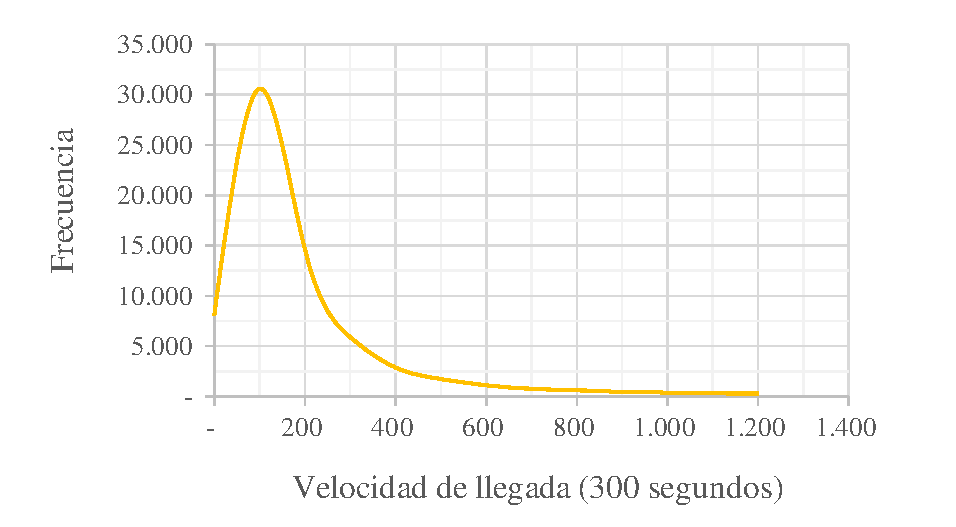
\includegraphics[trim={20 6 0 6}, clip, height=140pt]{imagenes/distribucion_02.pdf}
		\label{fig:data_distribution1}
	}\par\medskip
	\subfloat[b][Distribución del logaritmo de la frecuencia de los mensajes relacionados 
  		con sismos en ventanas de tiempo de 300 segundos.]{
  		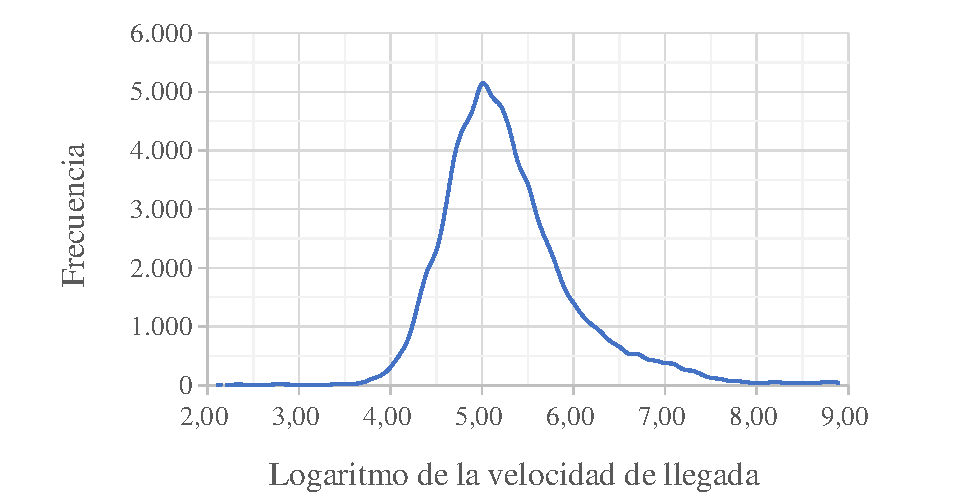
\includegraphics[trim={20 0 0 0}, clip, height=140pt]{imagenes/distribucion_03.pdf}
  		\label{fig:data_distribution2}
  	}
\end{wrapfigure}

La metodología propuesta se basa en monitorear el flujo de mensajes ($\mathcal{F}$) en el tiempo, para determinar cuándo una variación positiva en la velocidad de llegada relativa ($\lambda$) de elementos de interés es significativamente más grande que otras variaciones producidas por el ruido observado en el pasado.
%
Originalmente, en el método propuesto por Guzman y Poblete, la ``explosividad'' de cada palabra es estimada en base a la magnitud del cambio de su velocidad de llegada relativa ($\lambda$) con respecto a la ventana de tiempo previa.
%
La salida es una lista de los top-\emph{k} términos ordenados en orden decreciente según el cambio de su velocidad de llegada relativa ($\lambda$).
%
Esto no es suficiente para el propósito de la detección de sismos, ya que, como se detalló en la sección \ref{sec:recoleccion}, los datos que conforman el flujo fueron seleccionados a partir de palabras clave y datos geográficos. 
%
Ocasionando que, para este caso particular, se requiera monitorear un flujo sesgado en el que hay pocas palabras muy frecuentemente usadas (menos de \emph{k} palabras) y que experimentan pequeños cambios en cada ventana de tiempo debido a fluctuaciones al azar en los datos de entrada (i.e., ruido).
%
Por lo tanto, si se reportan las top-\emph{k} palabras más ``explosivas'' podría significar tener reportes en cada ventana de tiempo.
%
Es por esto, que para reportar sismos automáticamente se necesita estimar, de forma confiable, cuándo un cambio es significativo y por tanto indica actividad inusual.


El enfoque natural para determinar si la velocidad de llegada relativa ($\lambda$) experimenta una variación significativa durante una ventana de tiempo $w_i$ es monitorear la desviación estándar de $\lambda$ para todas las ventanas de tiempo hasta $w_{i-1}$; al igual que como se ha hecho en el trabajo previo sobre detección de eventos emergentes usando enfoques estadísticos basados en la distribución de frecuencias~\cite{kleinberg2003bursty, mathioudakis2010twittermonitor,
nguyen2013event}.
%
Esta idea asume y requiere que la velocidad de llegada relativa ($\lambda$) tenga una distribución exponencial. 
%
Sin embargo, un análisis empírico cuyo resultado se muestra en la figura ~\ref{fig:data_distribution1}, usando el conjunto de datos recolectados durante un periodo de 9 meses, desde el 25 de Enero al 25 de Octubre del 2016, indica que esto no se cumple para el caso de la distribución de la velocidad de llegada de las palabras relacionadas con sismos.
%
Esta observación hizo necesario un análisis para identificar como adaptar el algoritmo a los propósitos descritos en esta tesis.


Entre los análisis realizados hay uno en particular que resultó útil para continuar. Se aplicó una transformación logarítmica a los datos, tal como se muestra en la figura~\ref{fig:data_distribution2}, después de lo cual los datos se asemejan a una distribución {\em log-normal}.
%
Por lo tanto, en vez de monitorear los cambios en la velocidad relativa de llegada ($\lambda$), se modeló la distribución como si fuera {\em log-normal} y se monitorean los cambios en el logaritmo de la función. La función transformada se define como:

\begin{equation}
\label{eq:log_lambda}
\tilde{\lambda}(K, M_i) = \frac{\ln\left(\mathrm{freq}(K,M_i)\right)}{T |M_i|}
\end{equation}

Usando la función transformada $\tilde{\lambda}(K, M_i)$ se calculó su {\em z}-score\footnote{El z-score (standard score) indica a cuántas desviaciones estándar se encuentra un elemento de la media}. Este valor es monitoreado para identificar las variaciones significativas.  

\newcommand{\zscore}{\ensuremath{z\textnormal{-}\mathrm{score}}}
\begin{equation}
\label{eq:zscore}
\zscore(K, M_i) = \frac{\tilde{\lambda}(K, M_i)-\mu_i}{\sigma_i}
\end{equation}

\noindent donde $\mu_i$ y $\sigma_i$ son, respectivamente, el promedio y la desviación estándar de los valores observados de $\tilde\lambda$ durante las ventanas de tiempo $w_1, w_2, \dots, w_{i-1}$.

El método propuesto monitorea la señal discreta formada por los valores del {\em z}-score calculado para cada ventana de tiempo y catalóga como una detección de sismo cada uno de los instantes en donde $\zscore(K, M_i)\ge\theta$, donde $theta$ es un umbral definido experimentalmente.
%
En el capítulo~\ref{cap:analisis} se describen los experimentos realizados para determinar los parámetros iniciales y el valor del umbral para $\theta$. 
	
%\subsection{Metodología para ajustar los parámetros iniciales óptimos}
%
%La metodología de detección de sismos propuesta requiere que se fijen 3 parámetros iniciales:
%\begin{enumerate}
%\item El umbral para lanzar las alertas de detección de sismos $\theta$.
%\item La lista de atributos que definen un elemento de interés ($K$).
%\item El tamaño de cada ventana de tiempo ($T$).
%\end{enumerate}
%
%\medskip
%\noindent\textbf{(1) Umbral para detección de sismos ($\theta$):}
%%
%Para determinar las variaciones significativas en el flujo $\mathcal{F}$ se identificó el valor óptimo para el umbral $\theta$ empíricamente. 
%%
%Utilizando una muestra de datos de 2 meses, se probó el sistema de detección usando diferentes valores de $\theta$ y se seleccionó el valor que maximiza el F-measure.
%%
%La tabla~\ref{table:zscore} muestra los resultados obtenidos y el valor seleccionado $\theta=1.5$.
%\begin{table}
\centering
\begin{tabular}{cccc}
\toprule
{z-score ($\theta$)} & {Precision} & {Recall} & {F-Measure} \\ 
\midrule
{0.5}    & {48.1\%}     & {79.9\%}  & {60.1\%}  \\ 
{1.0}    & {62.6\%}     & {65.0\%}  & {63.8\%}  \\ 
{\bf 1.5}    & {\bf 88.3\%}     & {\bf 54.2\%}  & {\bf 67.1\%}  \\
{2.0}    & {92.3\%}     & {29.0\%}  & {44.2\%}  \\ 
\bottomrule
\end{tabular}
\caption{Comportamiento del algoritmo utilizando diferentes valores para el umbral de detecci\'on de sismos $\theta$.}
\label{table:zscore}
\end{table}

%
%
%\noindent\textbf{(2) Palabras clave relacionadas con sismos ($K$):} 
%Como se mencionó previamente, en esta adaptación los elementos de interés ($K$) son una lista de palabras clave relacionadas con la ocurrencia de sismos.
%%
%En esta tesis se extendió la lista de palabras entregada por investigadores del USGS, que fue usada en Earle et al.~\cite{earle2012twitter} y Avvenuti et al.~\cite{avvenuti2014earthquake,avvenuti2014ears}.
%%
%Sin embargo, a diferencia de los sistemas anteriores, la lista de palabras utilizada se construyó intentando incluir la mayor cantidad posible de palabras relacionadas con ocurrencias de sismos en cualquier idioma, incluso si incluía términos ambiguos (es decir, términos que a veces son utilizados en otros contextos).
%%
%Los mensajes ruidosos que puedan ser obtenidos al usar términos ambiguos no afectan el rendimiento de este método ya que es tolerante al ruido. 
%%
%Por ejemplo, la palabra ``quake'' puede ser usada para referirse a un videojuego o al personaje de un comic con el mismo nombre, o la palabra ``terremoto'' que en Chile también es utilizada para referirse a una bebida alcohólica típica y muy consumida durante las celebraciones nacionales. 
%%
%La lista de palabras está compuesta por los siguientes términos %{\em earthquake, sismo, quake, temblor, temblando, gempa, lindol, tremblement, erdbeben, deprem, seismós, séisme, zelzele, terremoto, scossa, bhukamp(sanskrit), \begin{CJK}{UTF8}{gbsn} 地震, 海啸, 津波, 地震, \end{CJK} \foreignlanguage{russian}{землетрясение}, \foreignlanguage{farsi}{زمین‌لرزه,زلزله}, \foreignlanguage{greek}{σεισμός}}
%%
%\jm{Agregar lista de palabras - Solucionar problema de codificación}
%Si se necesita agregar nuevos términos, la lista palabras puede ser actualizada dinámicamente.
%
%
%Además de las palabras clave relacionadas con sismos, se realizaron experimentos en los cuales además de las palabras clave, también se consideraban otros atributos para determinar si un elemento era de interés o no. 
%%
%De esta forma se pudo analizar la señal discreta asociada a diferentes tipos de atributos y determinar si estos agregaban valor a la detección o no. 
%%
%Entre estos atributos se encuentran:
%\begin{itemize}
%\item Sentimiento positivo del \textit{tweet}.
%\item Sentimiento negativo del \textit{tweet}.
%\item Idioma en el cual fue escrito el \textit{tweet}
%\item País mencionado en el texto del \textit{tweet}.
%\item País mencionado en la localidad de perfil del usuario que escribió el \textit{tweet}.
%\end{itemize}
%
%\begin{figure}[ht]
%  \centering
%  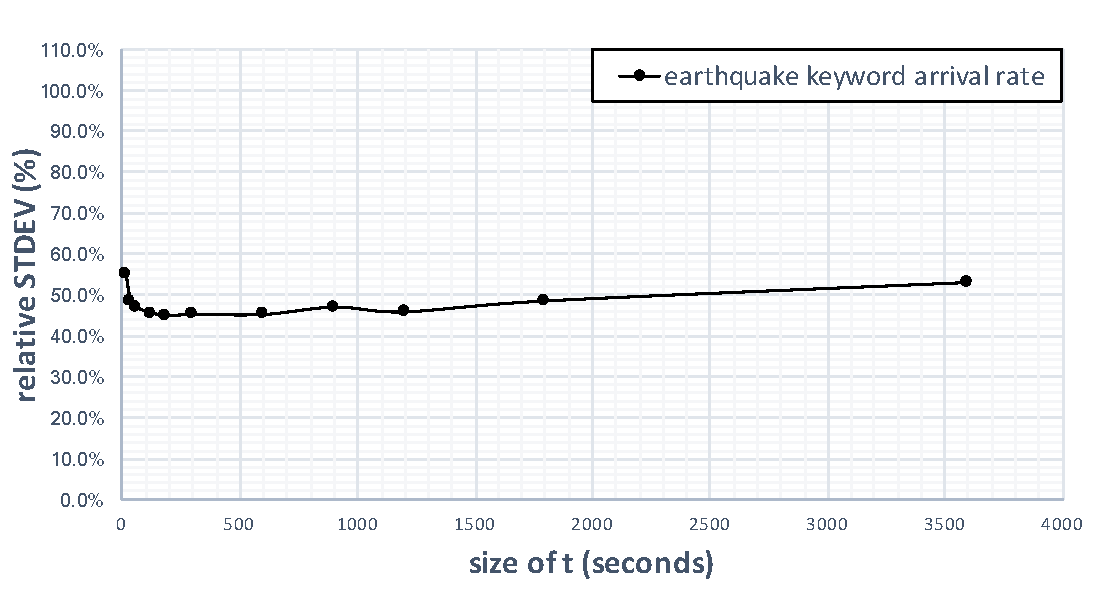
\includegraphics[trim={5 0 5 10}, clip, width=\textwidth]{imagenes/02_Poise_Analysis_WindowSize_solo.pdf}
%  \caption{Desviación estándar relativa de la señal que considera las palabras clave relacionadas con sismos para diferentes tamaños de ventana de tiempo (en segundos)}
%\label{fig:window_size}
%\end{figure}
%
%\noindent\textbf{(3) Tamaño de la ventana de tiempo ($T$):} 
%El tamaño de la ventana corresponde al largo del tiempo (en segundos) de cada conjunto de \textit{tweets} en los cuales son divididos los datos de la entrada para ser procesados por el algoritmo.
%%
%Este parámetro se determina analizando el flujo de la entrada y seleccionando un valor para $T$ que minimiza la desviación estándar relativa, es decir, cuando la frecuencia de aparición es más estable. 
%%
%Intuitivamente, si la ventana de tiempo es muy pequeña, los mensajes que contengan elementos en $K$ estarán distribuidos de forma más aleatoria en cada ventana. Esto significa que habrían ventanas de tiempo sin ninguna ocurrencia y otras con varias ocurrencias. Mientras más grande sea la ventana de tiempo, más factible es poder estimar la frecuencia en la ventana siguiente. 
%%
%Para determinar el valor de $T$ se utilizó el siguiente procedimiento, descrito en~\cite{guzman2013line}:
%%
%Para el flujo de entrada dado, se calcula la velocidad de llegada relativa de ventanas sucesivas $w_i$ de tamaño $T$.
%%
%Se repite este proceso para diferentes tamaños de ventana $T$ en el rango de $0$ hasta $3\,600$ segundos (una hora) para un periodo de 2 meses y se selecciona el $T$ con la desviación estándar relativa más pequeña. En este caso el valor de tamaño de ventana que minimiza la desviación estándar corresponde a los valores para $T \geq 300$ segundos, tal como se muestra en la figura~\ref{fig:window_size}.
%%
%Además, para disminuir los tiempos de detección, el sistema ejecuta dos procesos paralelos idénticos desfasados en $150$ segundos uno del otro y con ello asegurar un tiempo de detección de máximo 5 minutos. 
%
%%
%%In this experiment we
%%consider different possible input signals: 1) messages that contain an
%%earthquake keyword, 2) messages that contain an earthquake keyword and that
%%express positive sentiment\footnote{We extract the sentiment polarity of
%%Twitter messages using the off-the-shelf classifier SentiStrength
%%\url{http://sentistrength.wlv.ac.uk/}}, and 3) messages that
%%contain an earthquake keyword and that express negative sentiment. In our
%%experiment over a 2-month data stream we determine that the optimal
%%window-size must be greater than $120$ seconds, point at which the relative
%%standard deviation becomes stable.

\section{Análisis de Sentimiento}
\label{sec:sentimiento}

Uno de los objetivos específicos de esta tesis es la extracción de información u otros metadatos que permitan caracterizar los eventos sísmicos. 
%
Entre la información que se puede extraer de un \textit{tweet} se encuentra el análisis de sentimiento.
%
En particular en esta tesis se ejecutó una tarea básica en análisis de sentimientos que consiste en clasificar la polaridad de un texto.
%
Esta información fue utilizada para ver si al considerarlo dentro de los atributos de interés $K$ y analizar la señal asociada, mejoraba la detección cuando ocurría un sismo. 
%
La información queda almacenada en caso de ser útil en estudios posteriores que busquen estimar la intensidad de un evento o hacer otra especie de análisis. 


Para clasificar la polaridad del \textit{tweet} se utilizó el algoritmo SentiStreigth\footnote{\url{http://sentistrength.wlv.ac.uk}} con sus diccionarios específicos para diferentes lenguajes. 
%
Además se modificó el diccionario español agregando palabras pertenecientes al español ``chileno'' con el objetivo de mejorar la exactitud de la categorización en español.  


Dentro del conjunto de palabras que se agregaron del idioma español ``chileno'' se encuentran algunas utilizadas frecuentemente cuando se reporta un sismo y que denotan sorpresa, miedo o rabia, como improperios chilenos u otras expresiones comunes.
%
Además se agregaron palabras que denotan aprobación, como por ejemplo \textit{``bacán''}.


\section{Geocodificación de los datos}
\label{sec:geocodificacion}

Al recolectar los datos utilizando la API de Twitter se obtiene información asociada a cada \textit{tweet}. 
%
Esta información, en algunos casos, incluye información geográfica, dependiendo si el usuario tiene activado o no los mecanismos de geolocalización del dispositivo desde el cual publicó el mensaje.
%
El porcentaje de usuarios de Twitter que tienen activada la opción de compartir las coordenadas geográficas es muy bajo (cercano al 2\%) y varía dependiendo de cada país. 
%
Sin embargo, existen otros datos asociados a un \textit{tweet} que nos permiten inferir una posible ubicación desde la cual se publica ese mensaje. 
%
Estos datos no son 100\% confiables ni precisos y tampoco están disponibles para todos los \textit{tweets}, pero sin duda aumentan el porcentaje de \textit{tweets} para los cuales podemos aproximar una localidad llegando hasta un 80\%.


Las formas en que se obtuvo información relacionada a la localidad de un \textit{tweet} son:

\begin{enumerate}
\item Coordenadas GPS: Disponibles cuando el usuario tiene activado el mecanismo de GPS en su dispositivo y activada la opción que permite compartir estos datos en la red social.

\item Twitter Places: Cuando un usuario de Twitter escribe un mensaje asociado a algún lugar y tiene activado el GPS (no necesariamente permitiendo compartir las coodenadas), por ejemplo: \textit{``Que buen rato con amigas en el Starbucks''}. El dispositivo le sugiere al usuario agregar el lugar a partir de una lista de lugares que Twitter ya tiene almacenados, para este caso podría ser ``Starbucks Coffee, Agustinas, Santiago Centro, Santiago, Chile''. Si la persona acepta la sugerencia, esa información quedará asociada al \textit{tweet} y al ser un lugar que existe dentro de las bases de datos de Twitter, la información es muy completa.

\item Localidad del perfil del usuario: Cada usuario tiene la posibilidad de personalizar su perfil de Twitter. Entre los datos del perfil se encuentra información sobre su localidad, sin embargo, el usuario puede completar esta información ingresando texto libre. Como resultado, los usuarios escriben los nombres de los lugares de diferentes formas, con diferentes grados de precisión y por supuesto, también hay muchos nombres de lugares inexistentes o textos que no indican realmente dónde vive el usuario. A pesar de esto, este campo es muy utilizado por los usuarios de Twitter y en general si corresponde a información sobre un lugar real. 

\item Localidades mencionadas en el texto del \textit{tweet}: Al estar analizando \textit{tweets} que reportan sobre sismos, muchos de los mensajes incluyen nombres de localidades. Al igual que en el caso anterior, esta información puede estar escrita de diversas formas y siempre existe la posibilidad de que no sea información real. %Sin embargo esta información está presente en muchos de los mensajes y bajo el amparo de la ley de los grandes números, en esta tesis esta información también es considerada al momento de caracterizar un evento. 

\end{enumerate} 

Para extraer la información que se indica en los puntos 3. y 4. es necesario encontrar menciones de localidades en el texto disponible en el campo de localidad del usuario y en el corpus del \textit{tweet}. 
%
Para esto se utiliza un listado de nombre de países y sus traducciones a diferentes idiomas y un listado de ciudades chilenas que permite obtener información más detallada sobre localidades dentro de Chile. 
%
Para encontrar las menciones se analiza el texto buscando ocurrencias de países en primer lugar. Si el texto no contiene información de ningún país y el \textit{tweet} está escrito en español, se buscan nombres de ciudades chilenas. De la misma forma, para el caso de los \textit{tweets} escritos en japonés, se buscan nombres de ciudades de japón. 
%
Esto se puede extender para otros países de los cuales se quiera obtener información más detallada. Pero en esta tesis se evitó porque las coincidencias entre nombres de ciudades de diferentes países puede causar problemas en los resultados obtenidos. 
%
No se utilizó algo más sofisticado para extraer nombres de localidades debido a que estos datos tienen que ser procesados en tiempo real y no ocasionar cuellos de botella que retrasen los tiempos de la detección de sismos.

	
Una vez obtenidos los nombres de localidades, para información que se indica en los puntos 2, 3 y 4, es necesario además agregar coordenadas geográficas.
%
Para los casos en que solo se tiene información del país se les asignaron coordenadas genéricas en un punto céntrico del territorio. 
%
Para los casos en que hay información de las ciudades, se asignaron las coordenadas de la ciudad respectiva. 


\section{Visualización de datos}
\label{sec:visualizacion}
	\subsection{Temporales}
	
	\begin{figure}[ht]
	  \centering
	  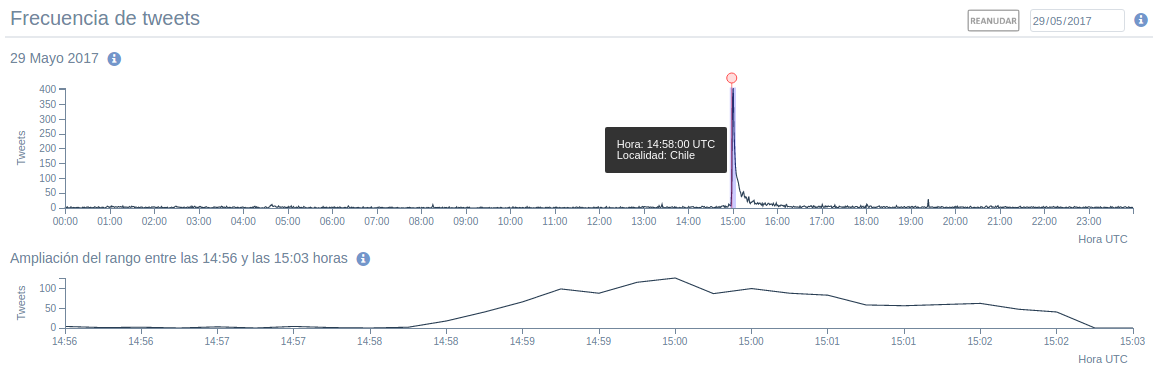
\includegraphics[trim={0 0 0 0}, clip, width=\textwidth]{imagenes/linea_de_tiempo_interactive.png}
	  \caption{Visualización de la frecuencia de \textit{tweets} de un día completo en intervalos de 60 segundos y de la frecuencia de \textit{tweets} de la zona seleccionada en intervalos de 15 segundos.}
	\label{fig:timeline}
	\end{figure}
		
	
	Para visualizar los datos temporales, se utiliza una señal interactiva similar a un gráfico de línea, que se actualiza a medida que pasa el tiempo y que muestra la cantidad de \textit{tweets} publicados en cada momento.
	%
	La imagen \ref{fig:timeline} corresponde a la visualización de los datos recolectados el día 29 de Mayo del 2017.
	%
	La primera señal muestra los datos recolectados en un rango de un día y la segunda señal muestra el rango seleccionado amplificado. Por defecto, están seleccionados los últimos 30 minutos.
		
	Mediante esta visualización es posible identificar rápidamente cambios en el comportamiento típico de los usuarios.
	%
	Además el sistema marca automáticamente los puntos de interés, en este caso, los puntos en donde inicia un sismo. 
	%
	Los usuarios pueden interactuar con esta visualización, ya sea seleccionando un rango de tiempo o haciendo \textit{click} en un punto de interés, lo que permite obtener información más detallada de el periodo de tiempo seleccionado. 
	
	
	\subsection{Geográficos}
	
	\begin{figure}[ht]
	\centering
	\subfloat[Mapa del mundo con \textit{tweets} geolocalizados.]{
		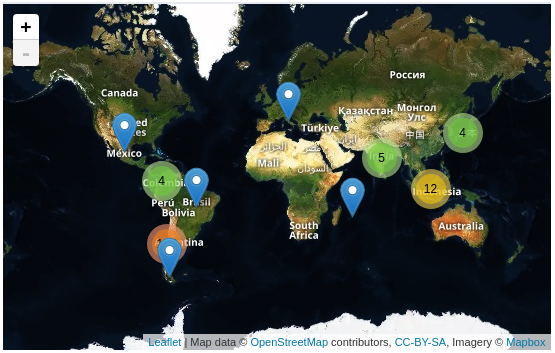
\includegraphics[height=140pt]{imagenes/worldmap.png}
		\label{fig:worldmap-out}
	}
	\hfill
	\subfloat[Mapa ampliado a la zona afectada por el sismo.]{
  		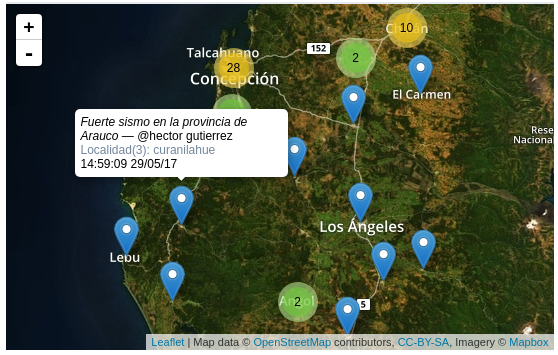
\includegraphics[height=140pt]{imagenes/worldmap-maxzoom.png}
  		\label{fig:worldmap-zoom}
  	}
  	\caption{Mapa interactivo con marcadores para cada tweet geolocalizado y agrupados en base a la distancia que existe entre ellos. Las imagenes corresponden a un sismo ocurrido cerca de  Concepción, Chile, el 29 de Mayo del 2017.}
  	\label{fig:worldmap}
  	\end{figure}
	 	
	  	
	Como se mencionó en la sección \ref{sec:geocodificacion} se intenta obtener la mayor cantidad posible de información geográfica. 
	%
	Esto es muy útil ya que, a pesar de no ser 100\% confiable, entrega una buena aproximación de la percepción de un sismo. 
	%
	Saber donde se encuentran los usuarios que reportan un sismo nos permite identificar las áreas afectadas y el alcance geográfico de cada evento. 
	%
	
	\begin{wrapfigure}{r}{0.4\textwidth}
	\vspace{-20px}
	  \centering
	  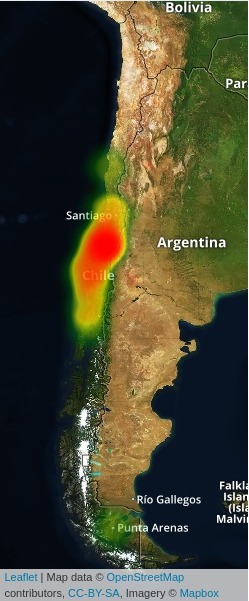
\includegraphics[trim={0 0 0 0}, clip, width=0.4\textwidth]{imagenes/heatmap.png}
	  \caption{Mapa de calor construido a partir de las coordenadas geográficas inferidas de los \textit{tweets} publicados durante un sismo en Concepción}
	\label{fig:heatmap}
	\vspace{-130px}
	\end{wrapfigure} 
	
	Para mostrar esta información se utilizan dos tipos de mapas, el primero consiste en un mapa de calor. 
	%
	La figura \ref{fig:heatmap} visualiza los datos recolectados durante los 15 minutos posteriores a un evento sísmico ocurrido el 29 de Mayo cerca de Concepción. 
	%
	En ella se puede observar la zona en donde se publicaron un mayor número de tweets y cómo esto se modifica en el tiempo.
	%
	%Como se puede observar, la imagen muestra una mancha roja un poco más abajo de Santiago. 
	%
	%Esto se debe a que este mapa no se encuentra normalizado. 
	%
	%Sin embargo el usuario tiene la opción de escoger ver el mapa normalizado por población regional, lo que permite observar más claramente que el evento ocurrió más al sur de Chile. 
	%
	%El mapa que muestra los mismos datos pero normalizados por región se muestra en la figura \ref{fig:heatmap-normalizado}.
	
	
	El segundo tipo de mapa consiste en un visualización interactiva del mapa del mundo con marcadores para cada tweet relacionado con alguna localización.
	%
	Para una mejor visualización, los datos se agrupan en base a su cercanía y se van separando en grupos más pequeños a medida que el usuario amplía el mapa o hace click en cada grupo. 
	%
	La figura \ref{fig:worldmap-out} muestra la visualización durante un sismo en Chile y la figura \ref{fig:worldmap-zoom} muestra el mismo instante pero con el mapa ampliado a la zona con mayor número de marcadores.
	%
	La visualización permite identificar rápidamente los lugares afectados, en este caso, en el mapa \ref{fig:worldmap-out} se identifica un grupo grande en Chile y a medida que se amplía esa zona, en el mapa \ref{fig:worldmap-zoom} se identifica un grupo numeroso en Concepción (ciudad muy cercana al epicentro) y las ciudades aledañas.
	
	
  	
\section{Aplicación Web}
\label{sec:aplicacion}

\subsection{Usuarios de la Aplicación}

Los usuarios finales de la aplicación son:

\begin{enumerate}
\item Sismólogos de las oficinas del Centro Sismológico Nacional de la Universidad de Chile (CSN)
\item Personas no expertas en sismología que deseen visitar el sitio Web
\end{enumerate}

\subsection{Diseño de la Aplicación}

El objetivo principal de la aplicación Web es presentar los datos a los usuarios expertos, es decir, a los sismólogos de las oficinas del CSN. 
%
La aplicación será visualizada en las pantallas de monitoreo ocupando pantallas ordenadas verticalmente, además se desea poder extraer la información relevante sin la necesidad de interacción.
%
Por otro lado, la aplicación que queda disponible para el resto de los usuarios debe ser fácil de comprender. 


Es de interés poder observar los datos en tiempo real y también se desea poder explorar la información de eventos pasados. 
%
Para cada evento se presenta información de geolocalización. 


Teniendo en cuenta los puntos antes mencionados se desarrollan dos vistas de la aplicación que presentan la misma información. 
% 
Las figuras \ref{fig:webapp} y \ref{fig:webapp_csn} muestran la vista de la aplicación disponible de manera pública y la utilizada por el CSN respectivamente. 
%
En ella se observan las visualizaciones descritas en la sección \ref{sec:visualizacion} y el listado de \textit{tweets}, que permite a los usuarios comprender mejor el evento. 

	\begin{figure}[ht]
	  \centering
	  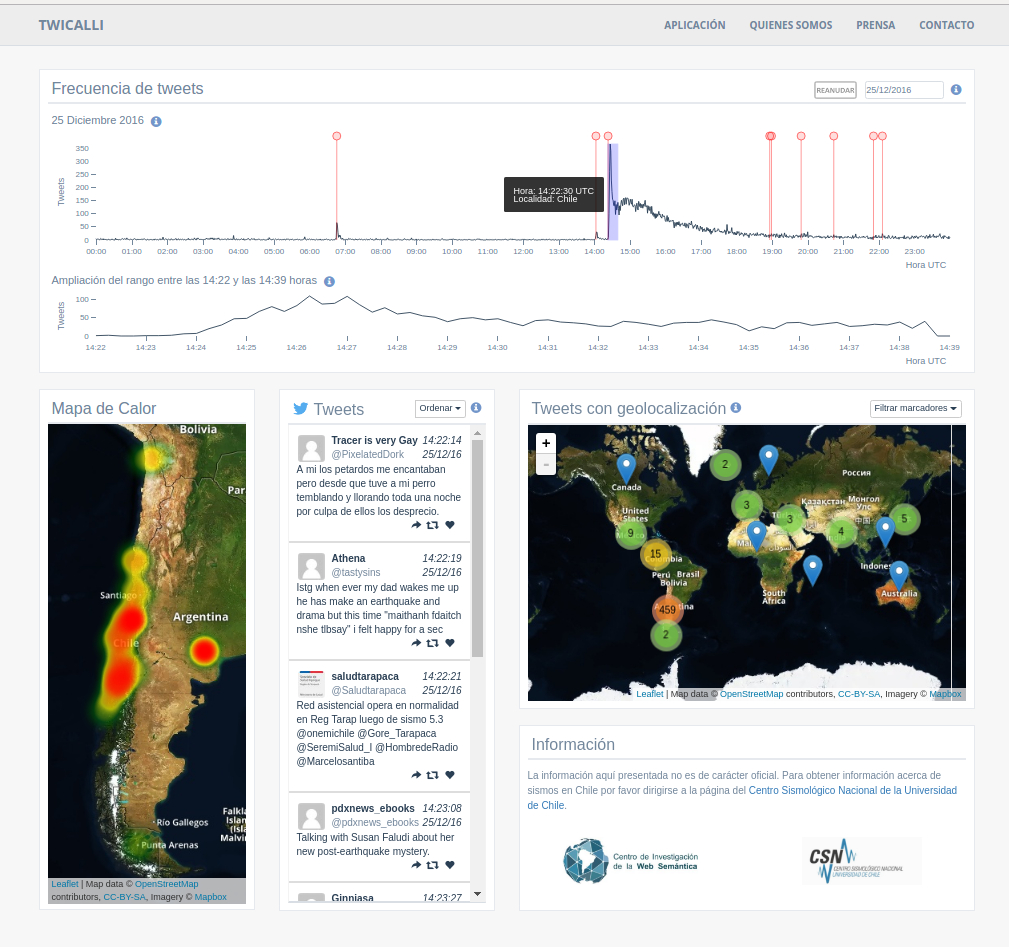
\includegraphics[trim={0 0 0 0}, clip, width=\textwidth]{imagenes/aplicacionexplorar.png}
	  \caption{Vista de la aplicación Web disponible públicamente}
	\label{fig:webapp}
	\end{figure}
	
	\begin{figure}[ht]
	  \centering
	  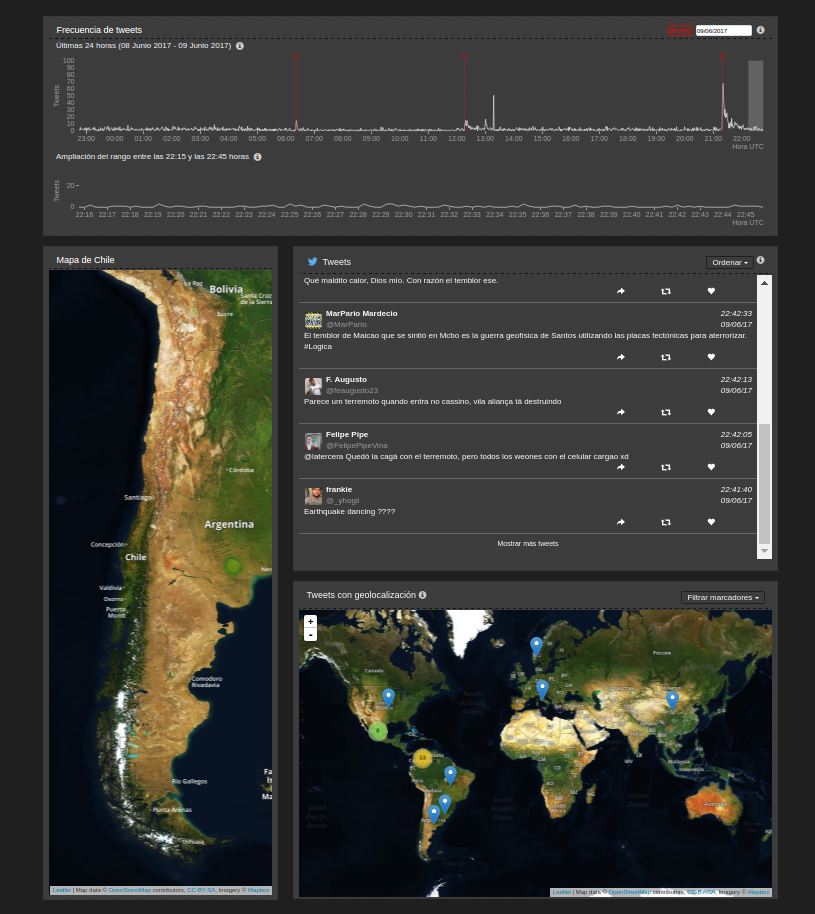
\includegraphics[trim={0 0 0 0}, clip, width=\textwidth]{imagenes/aplicacionexplorar_csn.png}
	  \caption{Vista de la aplicación Web utilizada por usuarios del CSN}
	\label{fig:webapp_csn}
	\end{figure}


Gracias a las iteraciones y la retroalimentación de los usuarios expertos se pudo identificar algunas mejoras, principalmente en la vista que visualizarán en las pantallas del CSN:

\begin{enumerate}
\item Preferencia por el uso de un mapa en el que se distinga el relieve del terreno y las fallas geográficas del borde costero chileno.
\item Selección de los colores utilizados en el mapa de calor y los marcadores para que no se confundan con los colores del mapa. 
\item Preferencia por el uso de una paleta de colores oscura para el fondo de la aplicación, debido a que el fondo blanco en las pantallas de monitoreo cansa la vista.
\end{enumerate}


\subsection{Interacciones}

La aplicación Web por defecto presenta los datos en tiempo real correspondiente a los últimos 30 minutos.
La línea de tiempo del día completo se actualiza cada 1 minuto y la línea de tiempo amplificada se actualiza cada 15 segundos. 
Además cada 1 segundo se consulta si hay nuevos \textit{tweets} y de ser así se dibujan en los mapas y en la parte superior de lista de tweets.  

Los usuarios pueden interactuar con la aplicación y en caso de hacerlo la actualización automática se detiene, pudiendo reanudarse en cualquier momento haciendo click en el botón \textit{reanudar} de la parte superior derecha de la línea de tiempo. 

Las interacciones disponibles son: 

\begin{itemize}
\item Seleccionar un largo de tiempo de la línea de tiempo principal. Esto permite actualizar la información en el resto de la página, mostrando el rango de tiempo amplificado y la información de los \textit{tweets} publicados durante ese rango de tiempo. 
\item Hacer click en un marcador rojo de la línea de tiempo principal, el cual representa la ocurrencia de un evento. Esta acción selecciona automáticamente el rango en el que aumentó el número de \textit{tweets} relacionados a ese evento y actualiza la información del resto de las visualizaciones de la misma forma que la interacción anterior. 
\item Hacer click en los marcadores del mapa que están agrupados para desagruparlos.
\item Hacer click en los marcadores desagrupados para mostrar información específica del \textit{tweet}.
\item Seleccionar una fecha para mostrar información de un día anterior. 
\end{itemize}



